\documentclass[conference]{IEEEtran}
\IEEEoverridecommandlockouts
% The preceding line is only needed to identify funding in the first footnote. If that is unneeded, please comment it out.
\usepackage{cite}
\usepackage{amsmath,amssymb,amsfonts}
\usepackage{graphicx}

\usepackage{filecontents}
\usepackage{algorithm}
\usepackage[end]{algpseudocode}
\usepackage[english]{babel}
\usepackage[utf8]{inputenc}

\begin{filecontents}{\jobname.bib}
@INBOOK{Singh2012,
author={Singh, S.
and Huang, K. L.
and Lin, B. S. P.},
title={An energy-efficient scheme for WiFi-capable M2M devices in hybrid LTE network},
booktitle={2012 IEEE International Conference on Advanced Networks and Telecommunciations Systems (ANTS)},
series={2012 IEEE International Conference on Advanced Networks and Telecommunciations Systems (ANTS)},
year={2012},
pages={126--130},
keywords={Long Term Evolution; wireless LAN; M2M devices; OPNET; WiFi; battery life; display technology; energy-efficient scheme; hand-held mobile devices; hybrid LTE network; machine to machine communication; power saving; processor power; storage capacity; LTE; Machine to Machine (M2M)},
issn={2153-1676},
doi={10.1109/ANTS.2012.6524242},
url={https://doi.org/10.1109/ANTS.2012.6524242}
}

@INBOOK{Tanaka2018,
author={Tanaka, K.
and Murase, M.
and Naito, K.},
title={Prototype implementation of BLE based automated data collection scheme in agricultural measurement system},
booktitle={2018 15th IEEE Annual Consumer Communications {\&} Networking Conference (CCNC)},
series={2018 15th IEEE Annual Consumer Communications {\&} Networking Conference (CCNC)},
year={2018},
pages={1--2},
keywords={Bluetooth; agriculture; computerised monitoring; measurement systems; mobile computing; smart phones; wireless LAN; wireless mesh networks; BLE; Bluetooth Low Energy; IEEE 802.15.4; agricultural measurement system; agricultural production; agricultural usages; automated data collection scheme; automated measurement information collection; background process; downward price trend; energy consumption; field sensing systems; mesh networks; mobile devices; power consumption reduction; recent systems; sensor devices; short range wireless communication technologies; smart data collection scheme; smartphone sensing; Cloud computing; Data collection; Market research; Semiconductor device measurement; Sensors; Wireless fidelity},
doi={10.1109/CCNC.2018.8319314},
url={https://doi.org/10.1109/CCNC.2018.8319314}
}

@INBOOK{Ng2013,
author={Ng, Ming Ann
and Yau, K. L. A.},
title={An energy-efficient Hybrid Wireless Mesh Protocol (HWMP) for IEEE 802.11s mesh networks},
booktitle={2013 IEEE International Conference on Control System, Computing and Engineering},
series={2013 IEEE International Conference on Control System, Computing and Engineering},
year={2013},
pages={17--21},
keywords={routing protocols; wireless mesh networks; IEEE 802.11s mesh networks; airtime metric; eHWMP; end-to-end delay; energy-efficient HWMP scheme; energy-efficient hybrid wireless mesh protocol; mobile nodes; packet error rate; path selection scheme; per-hop delay; residual energy; routing metric; throughput; transmission bitrate; Delays; Energy consumption; Energy efficiency; Energy states; IEEE 802.11 Standards; Routing; Energy-efficient; HWMP},
doi={10.1109/ICCSCE.2013.6719925},
url={https://doi.org/10.1109/ICCSCE.2013.6719925}
}

@INBOOK{Palan2017,
author={Palan, N. G.
and Barbadekar, B. V.
and Patil, S.},
title={Low energy adaptive clustering hierarchy (LEACH) protocol: A retrospective analysis},
booktitle={2017 International Conference on Inventive Systems and Control (ICISC)},
series={2017 International Conference on Inventive Systems and Control (ICISC)},
year={2017},
pages={1--12},
keywords={energy conservation; pattern clustering; routing protocols; wireless mesh networks; wireless sensor networks; HEEP; LEACH protocol; PEGASIS; TEEN; WSN; battery life; cluster based routing protocols; cluster head selection process; distributed mechanism; energy usage management; hybrid energy efficiency protocol; low energy adaptive clustering hierarchy protocol; multihop wireless network; threshold sensitive energy efficient network protocol; wireless sensor network; Batteries; Clustering algorithms; Control systems; Energy efficiency; Protocols; Steady-state; Faulty Sensor Node (FSN); LEACH; Sensor Node (SN); Wireless Sensor Network (WSN)},
doi={10.1109/ICISC.2017.8068715},
url={https://doi.org/10.1109/ICISC.2017.8068715}
}

@INBOOK{Sharma2006,
author={Sharma, G.
and Shroff, N. B.
and Mazumdar, R. R.},
title={Hybrid sensor and mesh networks: paradigms for fair and energy efficient communication},
booktitle={2006 2nd IEEE Workshop on Wireless Mesh Networks},
series={2006 2nd IEEE Workshop on Wireless Mesh Networks},
year={2006},
pages={83--92},
keywords={transceivers; wireless sensor networks; energy efficient communication; hybrid wireless sensor network; wireless communication capability; wireless mesh network; wireless transceiver; Batteries; Chemical sensors; Energy efficiency; IP networks; Intelligent networks; Mesh networks; Monitoring; Wireless communication; Wireless mesh networks},
doi={10.1109/WIMESH.2006.288604},
url={https://doi.org/10.1109/WIMESH.2006.288604}
}

@INBOOK{Haddad2009,
author={Haddad, E. C.
and Gregoire, J. C.},
title={Implementation issues for the deployment of a WMN with a hybrid fixed/cellular backhaul network in emergency situations},
booktitle={2009 1st International Conference on Wireless Communication, Vehicular Technology, Information Theory and Aerospace {\&} Electronic Systems Technology},
series={2009 1st International Conference on Wireless Communication, Vehicular Technology, Information Theory and Aerospace {\&} Electronic Systems Technology},
year={2009},
pages={525--529},
keywords={ad hoc networks; cellular radio; emergency services; radiofrequency interference; telecommunication network routing; telecommunication network topology; telecommunication traffic; wireless LAN; Lebanese territory; St-Joseph University; VoIP; WiFi hotspot; ad hoc wireless network; data communication; emergency situation; hybrid fixed/cellular back-haul network; mesh client; mesh router; priority traffic; radio interference; wireless mesh network; Admission control; Cellular networks; Collaboration; Communication system traffic control; Councils; Electromagnetic interference; Ground penetrating radar; Urban areas; Wireless mesh networks},
doi={10.1109/WIRELESSVITAE.2009.5172500},
url={https://doi.org/10.1109/WIRELESSVITAE.2009.5172500}
}


\end{filecontents}

\begin{document}

\title{Inserez un titre \\
\thanks{Identify applicable funding agency here. If none, delete this.}
}

\author{\IEEEauthorblockN{1\textsuperscript{st} Given Name Surname}
\IEEEauthorblockA{\textit{dept. name of organization (of Aff.)} \\
\textit{name of organization (of Aff.)}\\
City, Country \\
email address}
\and
\IEEEauthorblockN{2\textsuperscript{nd} Given Name Surname}
\IEEEauthorblockA{\textit{dept. name of organization (of Aff.)} \\
\textit{name of organization (of Aff.)}\\
City, Country \\
email address}
\and
\IEEEauthorblockN{3\textsuperscript{rd} Given Name Surname}
\IEEEauthorblockA{\textit{dept. name of organization (of Aff.)} \\
\textit{name of organization (of Aff.)}\\
City, Country \\
email address}
}

\maketitle

\begin{abstract}
Machine to Machine (M2M) communication has gained much interest in the recent past and the issues related to energy efficiency are central to all wireless networks, including wireless sensor, for an energy economy, we need to limit emissions so some nodes will make requests to their neighbors.  This article will show how to make sure neighbors are woken up during queries in a hybrid network architecture or how to make sure that the nodes that will receive the information will be woken up ?
\end{abstract}

\begin{IEEEkeywords}
M2M, hybrid network,hybrid network, wifi, ad-hoc
\end{IEEEkeywords}

\section{Introduction}


\section{Operation}
\begin{figure}[htbp]
\centerline{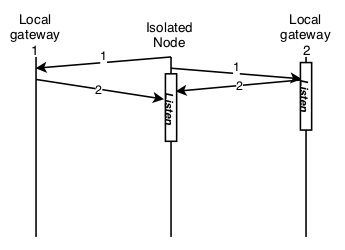
\includegraphics{discover.png}}
\caption{Discover Phase}
\label{fig1}
\end{figure}
Phase 1: Discovery 
Isolated nodes broadcast messages to discover(message 1) a Local Gateway. The end-nodes send messages every (X + random Integer) seconds. If a  Gateway receive a discovery message, the Local Gateway will accept (message 2 )and communicate to the end-nodes the communication slots.



\begin{figure}[htbp]
\centerline{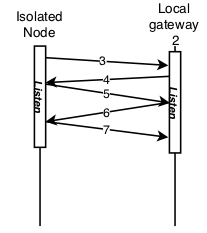
\includegraphics{register.png}}
\caption{Registering/pairing phase}
\label{fig2}
\end{figure}
Phase 2: Registration
 
The end-node will confirm the pairing to the Local gateway (message 3) . The end-node is registered to the Local gateway. 
There might be several Local gateway inside the system. However, there must never be multiple registrations on the same one.
After the local gateway receive the message 3, gateway send to the isolates node the message 4 to give his acknowledgment.
Message 5 is the first message from the isolated node, which contains datas to put an end the pairing phase. When all this stuff is done, the local gateway is able to send the message 6 : a request of data, then the node will answer his data.
 
\begin{figure}[htbp]
\centerline{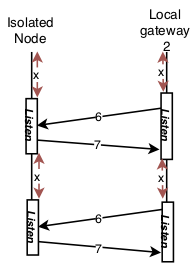
\includegraphics{harvest.png}}
\caption{harvest phase}
\label{fig3}
\end{figure}
Phase 3: Collection
The Local gateway will ask data to the end-nodes. If so, the isolated node sends the data to the Local gateway. This one will then forward it to another Gateway.
\newpage
\subsubsection{Accuracy}
Each message contains information on the next slot, the time of listening on this one, as well as the id of the senders and receivers. If a message is lost or collapsed, it will be re-sent managed by timers.

\subsubsection{Particular case}
When two gateways are in range from the isolated node and there both answer to him with the message 2. The isolated node pick one randomly.
To manage multiple isolated node, 
\section{Algorithm and simulation}
\subsection{Algorithm}

\subsubsection{Messages format}

The set of system messages are of the form:

\begin{center}
\texttt{< message\_type , source , destination , data >}
\end{center}

There are several messages in the system. It is considered that each message corresponds to a function carrying the name of the message, initializing the type and the source of the message, and taking in parameter the destination and the data.

\subsubsection{Message from IN to GW}
\begin{itemize}
    \item The \texttt{discover} message
    \begin{itemize}
      \item message set up for the discovery of a \texttt{GW} by an \texttt{IN}
      \item \texttt{destination = udef} :  broadcast mode
      \item \texttt{data = udef} : nothing
    \end{itemize}
    \item  Messages \texttt{pair}
    \begin{itemize}
      \item Pairing message from an IN to a GW.
      \item \texttt{data = udef} : nothing
    \end{itemize}
    \item Messages \texttt{data\_response}
    \begin{itemize}
      \item Answer from the data request of a GW.
    \end{itemize}
\end{itemize}

\subsubsection{les messages $GW \rightarrow IN$}
For all the messages coming from the \texttt{GW} the data part is structured as follows:

\begin{itemize}
  \item \texttt{answer\_frequency} : frequency on which the IN must respond
  \item \texttt{next\_slot} : delay by the next listening window
  \item \texttt{next\_duration} : fixed time of the next listening window
  \item \texttt{next\_frequency} : Frequency of the next listening window
  \item \texttt{data} : data space specific to the exchange
\end{itemize}

The message is like that   :

\begin{center}
\texttt{< message\_type , source , destination , answer\_frequency , next\_slot , next\_duration , next\_frequency , data>}
\end{center}

The different messages \texttt {GW} $ \ rightarrow $ \texttt {IN} are thus:
\begin{itemize}
     \item the messages \texttt {candidate} 
     \begin {itemize}
       \item \ texttt {GW} reply message after receiving \texttt{discover} from \texttt{IN}
       \item \ texttt {data = udef}: no info
     \end{itemize}
     \item messages \texttt{data\_request}
     \begin{itemize}
       \item data request message
       \item \texttt{data = udef} if only one data available or \texttt{data = requested\_data} in the case of multiple data
     \end{itemize}
\end {itemize}

\subsubsection{Liste des fonctions utilisées}

\paragraph{Fonction d'émission}

\texttt{void send(frequency , message)}

\paragraph{Fonction de réception}

la fonction \texttt{listen} écoute sur la fréquence \texttt{frequency} un temps définit par \texttt{time}. Le prototype de cette fonction est :

\begin{center}
\texttt{(message,time) listen(frequency , source , message\_type , time\_listen)}
\end{center}

les valeurs des paramètres de cette fonction sont :
\begin{itemize}
  \item \texttt{frequency} : fréquence d'écoute
  \item \texttt{source} : id de l'émetteur du message
  \begin{itemize}
    \item \texttt{source = udef} : écoute de tous les n{\oe}uds sur la fréquence définie
  \end{itemize}
  \item \texttt{message\_type} : type de message attendu
  \begin{itemize}
    \item \texttt{message\_type = udef} : écoute de tous les types de messages
  \end{itemize}
  \item \texttt{time\_listen} : durée de la fenêtre de réception
  \begin{itemize}
    \item \texttt{time\_listen = udef} : fenêtre infinie
  \end{itemize}
\end{itemize}

Valeurs de retour :

\begin{itemize}
  \item \texttt{message} message reçu
  \begin{itemize}
    \item passage du message dans sa totalité
    \item \texttt{message == udef} : pas de réception respectant les contraintes
  \end{itemize}
  \item \texttt{time} temps restant basé sur \texttt{time\_listen}
  \begin{itemize}
    \item \texttt{time == udef} : dans le cas de \texttt{time\_listen = udef}
  \end{itemize}
\end{itemize}
\newpage
\subsubsection{Algorithm 1 - 1}

\paragraph{Algorithm des \texttt{IN}}

\begin{algorithm}[!h]
\caption{Initialization of communication variables of IN}\label{alg:intvar}
\begin{algorithmic}[1]
\Procedure{$init\_var$}{msg}
\State $gw \leftarrow msg.source$
\State $next\_time \leftarrow msg.next\_slot$
\State $timer \leftarrow msg.next\_duration$
\EndProcedure
\State
\Procedure{$flush\_var$}{~}
\State $gw \leftarrow udef$
\State $msg \leftarrow udef$
\State $next\_time \leftarrow udef$
\State $timer \leftarrow timer\_disco$
\EndProcedure
\end{algorithmic}
\end{algorithm}
%Lorem ipsum dolor sit amet, consectetur adipiscing elit. Aenean viverra nunc augue, in interdum dolor vehicula nec. Mauris pulvinar urna quis elit mattis tincidunt. Pellentesque aliquam ipsum vitae urna vulputate, vel auctor dui tincidunt. Cras vehicula quam eget tellus condimentum, ut tincidunt mi lobortis. Vestibulum ac sem sit amet velit pellentesque euismod id ut sapien. Donec ac porta lorem. Phasellus euismod blandit mattis. Proin magna lorem, bibendum vel libero in, sollicitudin imperdiet lacus. Curabitur eget arcu risus. Cras vitae maximus magna, sit amet gravida ipsum. Vivamus malesuada leo id dui mattis efficitur.



\begin{algorithm}
\caption{Algorithm IN 1-1}\label{alg:in1-1}
\begin{algorithmic}[1]
\While{$(true)$}
  \State $flush\_var()$
  %\State \Comment{------------------------------------------------------- \textit{phase d'apairage}}
  \While{$(msg = udef)$}
    \State $send(freq\_listen,discover(udef,udef))$
    \State $(msg,t) = listen(udef,candidate,timer +rnd())$
  \EndWhile
  \State $initVar(msg)$
  \State $send(freq\_send,pair(gw,udef))$
  \State
  %\State \Comment{----------------------------------------------\textit{Phase d'échanges}}
  \While{$(gw != udef)$}
    \State $sleep(next\_time)$
    \State $(msg,t) = listen(gw,data\_request,timer)$
    \If{$msg != udef$}
      \State $initVar(msg)$
      \State $send(fdate\_response(gw,local\_data)$
    \Else
      $flush\_var()$
    \EndIf
  \EndWhile
\EndWhile
\end{algorithmic}
\end{algorithm}
%Lorem ipsum dolor sit amet, consectetur adipiscing elit. Aenean viverra nunc augue, in interdum dolor vehicula nec. Mauris pulvinar urna quis elit mattis tincidunt. Pellentesque aliquam ipsum vitae urna vulputate, vel auctor dui tincidunt. Cras vehicula quam eget tellus condimentum, ut tincidunt mi lobortis. Vestibulum ac sem sit amet velit pellentesque euismod id ut sapien. Donec ac porta lorem. Phasellus euismod blandit mattis. Proin magna lorem, bibendum vel libero in, sollicitudin imperdiet lacus. Curabitur eget arcu risus. Cras vitae maximus magna, sit amet gravida ipsum. Vivamus malesuada leo id dui mattis efficitur.


\subsubsection{Algorithm  of \texttt{GW}}

\begin{algorithm}
\caption{Initialization of communication variables of GW}\label{alg:initvarlg}
\begin{algorithmic}[1]
\Procedure{$init\_var$}{~}
\State $freq\_send \rightarrow chose()$
\State $timer \leftarrow chose()$
\State $freq\_listen \leftarrow chose()$
\State $freq\_next \leftarrow chose()$
\EndProcedure
\State
\Procedure{$flush\_var$}{~}
\State $timer \leftarrow timer\_disco$
\State $freq\_listen \leftarrow freq\_disco$
\State $freq\_send \leftarrow freq\_disco$
\State $in \leftarrow udef$
\EndProcedure
\end{algorithmic}
\end{algorithm}
%Lorem ipsum dolor sit amet, consectetur adipiscing elit. Aenean viverra nunc augue, in interdum dolor vehicula nec. Mauris pulvinar urna quis elit mattis tincidunt. Pellentesque aliquam ipsum vitae urna vulputate, vel auctor dui tincidunt. Cras vehicula quam eget tellus condimentum, ut tincidunt mi lobortis. Vestibulum ac sem sit amet velit pellentesque euismod id ut sapien. Donec ac porta lorem. Phasellus euismod blandit mattis. Proin magna lorem, bibendum vel libero in, sollicitudin imperdiet lacus. Curabitur eget arcu risus. Cras vitae maximus magna, sit amet gravida ipsum. Vivamus malesuada leo id dui mattis efficitur.


\begin{algorithm}[H]
\caption{Algorithm gw 1-1}\label{alg:gw1-1}
\begin{algorithmic}[1]
\State $LoRaWAN\_join()$
\State $flush\_var()$
\While{$(true)$}
  \If{$(in == udef)$}
    \State $(msg,t) = listen(,udef,discover,timer)$
  \EndIf
  \If{$(msg != udef)$}
    \State $in \leftarrow msg.source$
    \State $init\_var()$
    \State $send(candidate(in,slot,duration,udef)$
    \State $(msg,t) = listen(,in,pair,timer)$
    \If{$(msg == udef)$}
      \State $flush\_var()$
    \EndIf
  \EndIf
  \If{$(in != udef)$}
    \State $init\_var()$
    \State $send(data\_request(in,slot,durationt,udef)$
    \State $(msg,t) = listen(in,data\_response,timer)$
    \If{$(msg != udef)$}
      \State $send\_data(id + ":" + local\_data + ";" + in + ":" + msg.data)$
    \Else
      \State $send\_data(id + ":" + local\_data + ";" + in + ":" + udef)$
      \State $flush\_var()$
    \EndIf
  \EndIf
\EndWhile
\end{algorithmic}
\end{algorithm}


%Lorem ipsum dolor sit amet, consectetur adipiscing elit. Aenean viverra nunc augue, in interdum dolor vehicula nec. Mauris pulvinar urna quis elit mattis tincidunt. Pellentesque aliquam ipsum vitae urna vulputate, vel auctor dui tincidunt. Cras vehicula quam eget tellus condimentum, ut tincidunt mi lobortis. Vestibulum ac sem sit amet velit pellentesque euismod id ut sapien. Donec ac porta lorem. Phasellus euismod blandit mattis. Proin magna lorem, bibendum vel libero in, sollicitudin imperdiet lacus. Curabitur eget arcu risus. Cras vitae maximus magna, sit amet gravida ipsum. Vivamus malesuada leo id dui mattis efficitur.


\subsection{Simulation}

\newpage
\section{Conclusion}
\cite{Tanaka2018},
\cite{Singh2012},
\cite{Ng2013},
\cite{Palan2017},
\cite{Sharma2006},
\cite{Haddad2009}
\section*{Acknowledgment}


\bibliographystyle{plain}
\bibliography{article}
%\bibliography{article} 
%\bibliography{sample} 
\end{document}
